\Ac{mri} provides promising imaging techniques to overcome the drawbacks of
current clinical screening techniques mentioned in \acs{sec}\,\ref{chap:1}.
Unlike \ac{trus} biopsy, \ac{mri} examination is a non-invasive protocol and
has been shown to be the most accurate and harmless technique currently
available~\cite{Turkbey2012}.
In this section, we review different \ac{mri} imaging techniques developed for
\ac{cap} detection and diagnosis.
Features strengthening each modality will receive particular attention together
with their drawbacks.
Commonly, these features form the basis for developing analytic tools and
automatic algorithms.
However, we refer the reader to
\acs{sec}\,\ref{subsec:chp3:img-clas:CADX-fea-dec} for more details on
automatic feature detection methods since they are part and parcel of the
\acs{cad} framework.

\begin{figure}
  \centering
  \hspace*{\fill}
  \subfloat[\acs*{t2w}-\acs*{mri} slice of a healthy prostate acquire with a
  \SI{1.5}{\tesla} \acs*{mri} with an endorectal coil. The blue contour
  represents the \acs*{cg} while the \acs*{pz} corresponds to the green
  contour.]{\label{subfig:t2whealthy}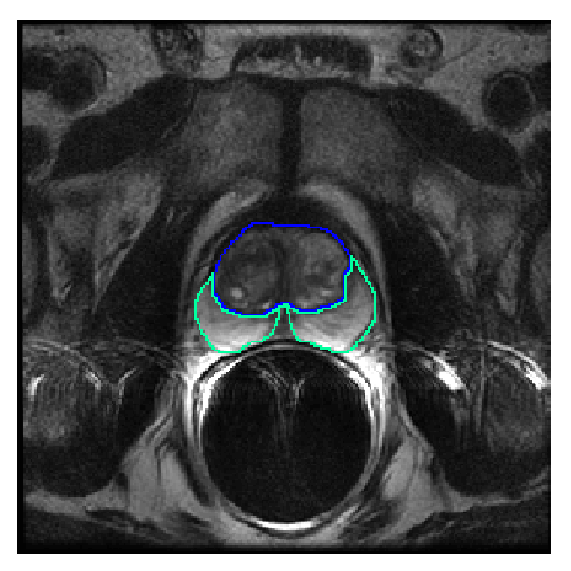
\includegraphics[width=0.3\linewidth]{2_modality/figures/t2w/t2w_healthy.eps}}
  \hfill
  \subfloat[\acs*{t2w}-\acs*{mri} slice of a prostate with a \acs*{cap}
  highlighted in the \acs*{pz} using a \SI{3}{\tesla} \acs*{mri} scanner
  without an endorectal
  coil.]{\label{subfig:t2wcancerpz}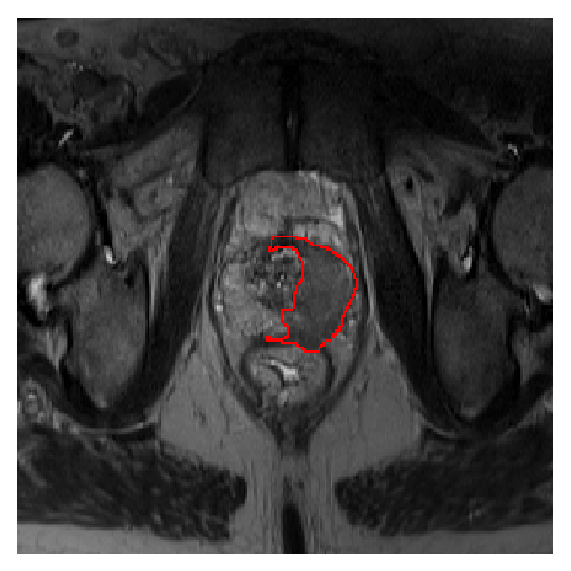
\includegraphics[width=0.3\linewidth]{2_modality/figures/t2w/t2w_cancer_pz.eps}}
  \hfill
  \subfloat[\acs*{t2w}-\acs*{mri} slice of a prostate with a \acs*{cap}
  highlighted in the \acs*{cg} using a \SI{1.5}{\tesla} \acs*{mri} scanner with
  an endorectal
  coil.]{\label{subfig:t2wcancercg}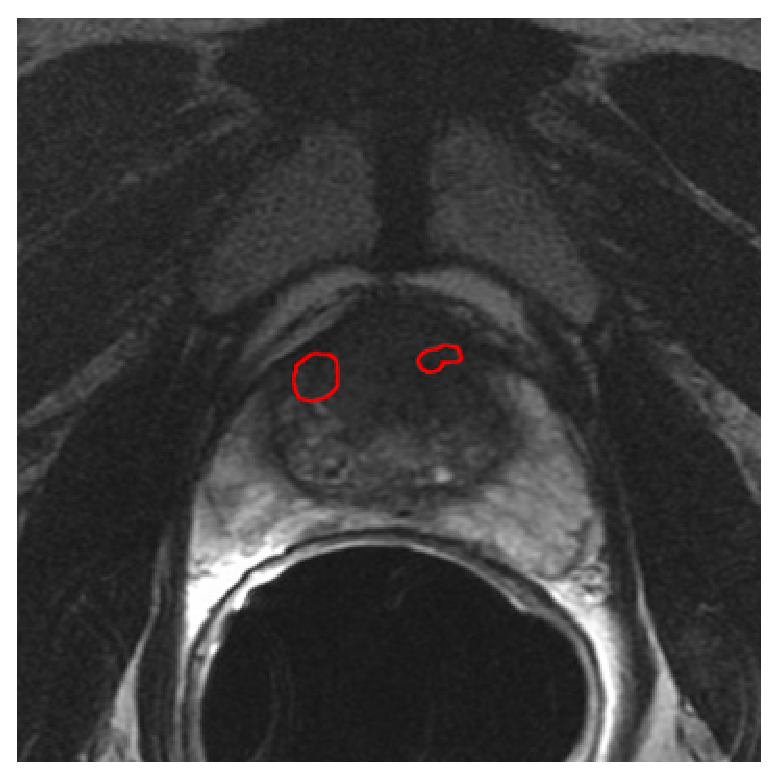
\includegraphics[width=0.3\linewidth]{2_modality/figures/t2w/t2w_cancer_cg.eps}}
  \hspace*{\fill}
  \caption[Rendering of \acs*{t2w}-\acs*{mri} prostate images.]{Rendering of
    \acs*{t2w}-\acs*{mri} prostate image with both \SI{1.5}{\tesla} and
    \SI{3}{\tesla} \acs*{mri} scanner.}
  \label{fig:t2w}
\end{figure}

\subsection{\acs*{t2w}-\acs*{mri}}\label{subsec:chp2:imaging:t2w}
\ac{t2w}-\ac{mri} has been the first \ac{mri}-modality used to perform \ac{cap}
diagnosis using \ac{mri}~\cite{Hricak1983}.
Nowadays, radiologists make use of it for \ac{cap} detection, localization, and
staging purposes.
This imaging technique is well suited to render zonal anatomy of the
prostate~\cite{Barentsz2012}.

This modality relies on a sequence based on setting a long \ac{tr}, reducing
the T$_{1}$ effect in \ac{nmr} signal measured, and fixing the \ac{te} to
sufficiently large values in order to enhance the T$_{2}$ effect of tissues.
Thus, \ac{pz} and \ac{cg} tissues are well perceptible in these images.
The former is characterized by an intermediate/high-\ac{si} while the latter is
depicted by a low-\ac{si}~\cite{Hricak1987}.
An example of a healthy prostate is shown in \acs{fig}\,\ref{subfig:t2whealthy}.

In \ac{pz}, round or ill-defined low-SI masses are synonymous with
\acp{cap}~\cite{Hricak1983} as shown in \acs{fig}\,\ref{subfig:t2wcancerpz}.
Detecting \ac{cap} in \ac{cg} is more challenging.
Both normal \ac{cg} tissue and malignant tissue, have a low-\ac{si} in
\ac{t2w}-\ac{mri}, reinforcing difficulties to distinguish one among them.
However, \acp{cap} in \ac{cg} appear often as homogeneous mass having
ill-defined edges with lenticular or ``water-drop''
shapes~\cite{Akin2006,Barentsz2012} as depicted in
\acs{fig}\,\ref{subfig:t2wcancercg}.

\ac{cap} aggressiveness has been shown to be inversely correlated with \ac{si}.
Indeed, \acp{cap} assessed with a \ac{gs} of 4-5 implied lower \ac{si} than the
one with a \ac{gs} of 2-3~\cite{Wang2008}.

In spite of the availability of these useful and encouraging features, the
\ac{t2w} modality lacks reliability~\cite{Kirkham2006,Hoeks2011}.
Sensitivity is affected by the difficulties in detecting cancers in
\ac{cg}~\cite{Kirkham2006} while specificity rate is highly affected by
outliers~\cite{Barentsz2012}.
In fact, various conditions emulate patterns of \ac{cap} such as \ac{bph},
post-biopsy hemorrhage, atrophy, scars, and
post-treatment~\cite{Hricak1987,Quint1991,Scheidler1999,Cruz2002,Barentsz2012}.
These issues are partly addressed using more innovative and advanced modalities.

% T2 Map
\subsection{T$_2$ map} \label{subsec:chp2:imaging:t2}
As previously mentioned, \ac{t2w}-\ac{mri} modality shows low sensitivity.
Moreover, \ac{t2w}-\ac{mri} images are a composite of multiple
effects~\cite{Hegde2013}.
However, T$_2$ values alone have been shown to be more
discriminative~\cite{Liu2011} and highly correlated with citrate concentration,
a biological marker in \ac{cap}~\cite{Liney1996,Liney1997}.
T$_2$ values are computed using the characteristics of transverse relaxation
which is formalized as in \acs{eq}\,\eqref{eq:tramag}.

\begin{equation}
  M_{xy}(t) = M_{xy}(0) \exp \left( - \frac{t}{\text{T}_2} \right) \ ,
  \label{eq:tramag}
\end{equation}

\noindent where $M_{xy}(0)$ is the initial value of $M_{xy}(t)$ and T$_2$ is
the relaxation time.

By rearranging \acs{eq}\,\eqref{eq:tramag}, T$_2$ map is computed by performing
a linear fitting on the model presented in \acs{eq}\,\eqref{eq:t2map} using
several TE, $t=\{ \text{TE}_1,\text{TE}_2, \dotsc ,\text{TE}_m \}$.

\begin{equation}
  \ln \left[ \frac{M_{xy}(t)}{M_{xy}(0)} \right] = - \frac{t}{\text{T}_2} \ .
  \label{eq:t2map}
\end{equation}

The \Ac{fse} sequence has been shown to be particularly well suited in order to
build a T$_2$ map and obtain accurate T$_2$ values~\cite{Liney1996a}.
Similar to \ac{t2w}-\ac{mri}, T$_2$ values associated with \ac{cap} are
significantly lower than those of healthy tissues~\cite{Liney1996,Gibbs2001}.

\begin{figure}
  \centering
  \hspace*{\fill}
  \subfloat[\acs*{t1w}-\acs*{mri} image where the cancer is delimited by the
  red contour. The green area was still not invaded by the
  \acs*{cap}]{\label{subfig:t1w}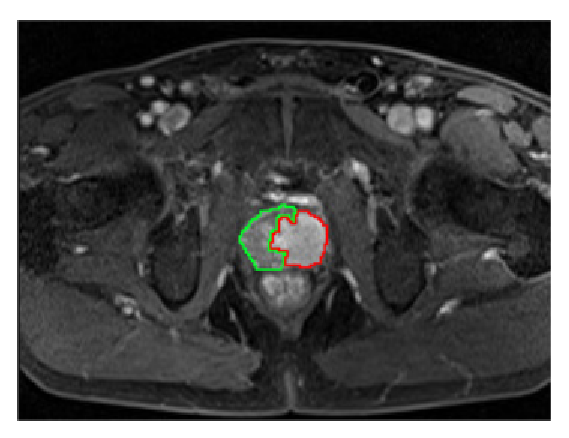
\includegraphics[width=0.4\linewidth]{2_modality/figures/dce/slice.eps}}
  \hfill
  \subfloat[Enhancement curve computed during the \acs*{dce}-\acs*{mri}
  analysis. The red curve is typical from \acs*{cap} cancer while the green
  curve is characteristic of healthy
  tissue.]{\label{subfig:dce}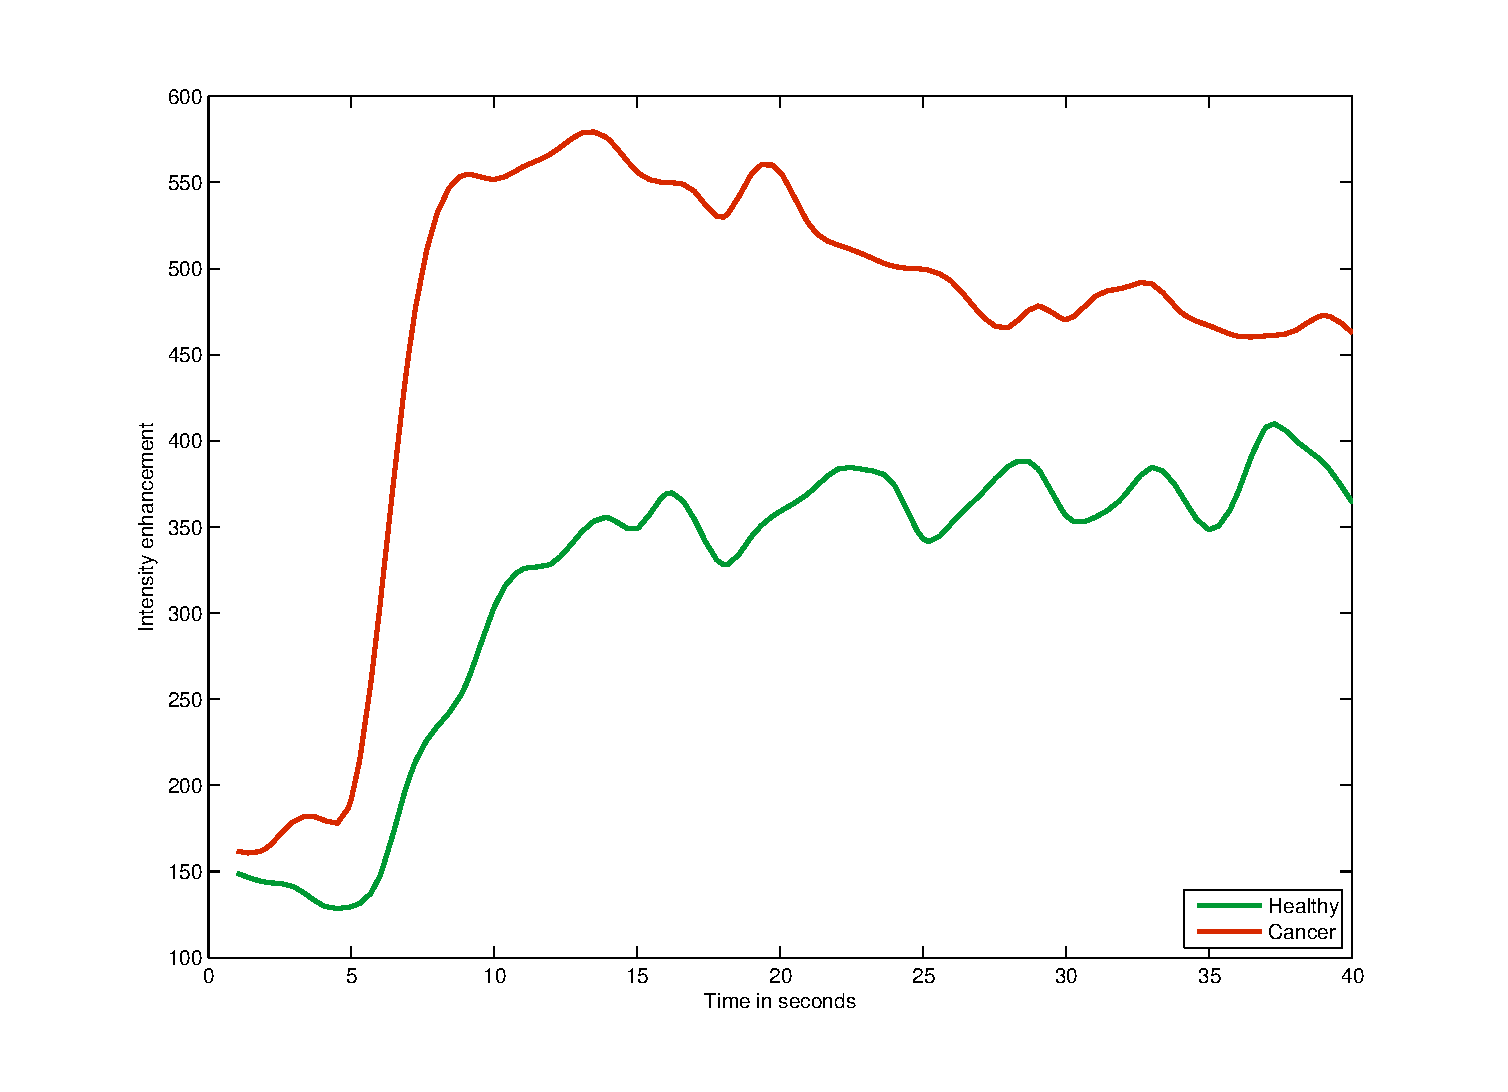
\includegraphics[width=0.45\linewidth]{2_modality/figures/dce/dce_cancer_healthy.eps}}
  \hspace*{\fill}
  \caption[Enhancement of \acs*{dce}-\acs*{mri} signal.]{Illustration of
    typical enhancement signal observed in \acs*{dce}-\acs*{mri} analysis
    collected with a \SI{3}{\tesla} \acs*{mri} scanner.}
  \label{fig:dceana}
\end{figure}

\subsection{\acs*{dce}-\acs*{mri}}\label{subsec:chp2:imaging:dce}
\Ac{dce}-\ac{mri} is an imaging technique which exploits the vascularity
characteristic of tissues.
Contrast media, usually gadolinium-based, is injected intravenously into the
patient.
The media extravasates from vessels to \ac{ees} and is released back into the
vasculature before being eliminated by the kidneys~\cite{Gribbestad2005}.
Furthermore, the diffusion speed of the contrast agent may vary due to several
parameters: the permeability of the micro-vessels, their surface area,
and the blood flow~\cite{Padhani2002}.

Healthy \ac{pz} is mainly made up of glandular tissue, around
\SI{70}{\percent}~\cite{Choi2007}, which implies a reduced interstitial space
restricting exchanges between vessels and
\ac{ees}~\cite{Buckley2004,Niekerk2009}.
Normal \ac{cg} has a more disorganized structure, composed of mainly fibrous
tissue~\cite{Choi2007,Hoeks2011}, which facilitates the arrival of the contrast
agent in \ac{ees}~\cite{Niekerk2013}.
To understand the difference between contrast media kinetic in malignant
tumours and the two previous behaviours mentioned, one has to focus on the
process known as angiogenesis~\cite{Carmeliet2000}.
In order to ensure growth, malignant tumours produce and release angiogenic
promoter substances~\cite{Carmeliet2000}.
These molecules stimulate the creation of new vessels towards the
tumour~\cite{Carmeliet2000}.
However, the new vessel networks in tumours differ from those present in
healthy tissue~\cite{Gribbestad2005}.
They are more porous due to the larger number of ``openings'' in their
capillary walls~\cite{Gribbestad2005,Choi2007}.
In contrast to healthy cases, this increased vascular permeability results in
increased contrast agent exchanges between vessels and
\ac{ees}~\cite{Verma2012}.

By making use of the previous aspects, \ac{dce}-\ac{mri} is based on an
acquisition of a set of \ac{t1w}-\ac{mri} images over time.
The gadolinium-based contrast agent shortens T$_1$ relaxation time enhancing
contrast in \ac{t1w}-\ac{mri} images.
The aim is to post-analyze the pharmacokinetic behaviour of the contrast media
concentration in prostate tissues~\cite{Verma2012}.
The image analysis is carried out in two dimensions: (i) in the spatial domain
on a pixel-by-pixel basis and (ii) in the time domain corresponding to the
consecutive images acquired with the \ac{mri}.
Thus, for each spatial location, a signal linked to contrast media
concentration is measured as shown in
\acs{fig}\,\ref{subfig:dce}~\cite{Tofts2010}.

By taking the above remarks into account, \acp{cap} is characterized by a
signal having an earlier and faster enhancement and an earlier wash-out ---
i.e, the rate of the contrast agent flowing out of the tissue --- as shown in
\acs{fig}\,\ref{subfig:dce}~\cite{Verma2012}.
Three different approaches exist to analyze these signals with the aim of
labelling them as corresponding to either normal or malignant tissues.

Qualitative analysis is based on a qualitative assessment of the signal
shape~\cite{Hoeks2011}.
Quantitative approaches consist of inferring pharmocokinetic parameter
values~\cite{Tofts2010}.
Those parameters are part of mathematical-pharmacokinetic models which are
directly based on physiological exchanges between vessels and \ac{ees}.
Several pharmacokinetic models have been proposed such as the Kety
model~\cite{Kety1951}, the Tofts model~\cite{Tofts1997}, and mixed
models~\cite{Larsson1996,StLawrence1998}.
The last family of methods mixed both approaches and are grouped together under
the heading of semi-quantitative methods.
They rely on shape characterization using mathematical modelling to extract a
set of parameters such as wash-in gradient, wash-out, integral under the curve,
maximum signal intensity, time-to-peak enhancement, and start of
enhancement~\cite{Hoeks2011,Verma2012}.
These parameters are depicted in \acs{fig}\,\ref{fig:dceparam}.
It has been shown that semi-quantitative and quantitative methods improve
localization of \ac{cap} when compared with qualitative
methods~\cite{Rosenkrantz2013}.
\Ac{sec}~\ref{subsubsec:chp3:img-clas:CADX-fea-dec:DCE-fea} provides a full
description of quantitative and semi-quantitative approaches.

\ac{dce}-\ac{mri} combined with \ac{t2w}-\ac{mri} has shown to enhance
sensitivity compared to \ac{t2w}-\ac{mri}
alone~\cite{Jager1997,Kim2005,Schlemmer2004,Zelhof2009}.
Despite this fact, \ac{dce}-\ac{mri} possesses some drawbacks.
Due to its ``dynamic'' nature, patient motions during the image acquisition
lead to spatial mis-registration of the image set~\cite{Verma2012}.
Furthermore, it has been suggested that malignant tumours are difficult to
distinguish from prostatitis located in \ac{pz} and \ac{bph} located in
\ac{cg}~\cite{Hoeks2011,Verma2012}.
These pairs of tissues tend to have similar appearances.
Later studies have shown that \acp{cap} in \ac{cg} do not always manifest in
homogeneous fashion.
Indeed, tumours in this zone can present both hypo-vascularization and
hyper-vascularization which illustrates the challenge of \ac{cap} detection in
\ac{cg}~\cite{Niekerk2013}.

\begin{figure}
  \centering
  \hspace*{\fill}
  \subfloat[\acs*{dw}-\acs*{mri} image acquired with a \SI{1.5}{\tesla}
  \acs*{mri} scanner. The cancer corresponds to the high \acs*{si} region
  highlighted in
  red.]{\label{subfig:dwi}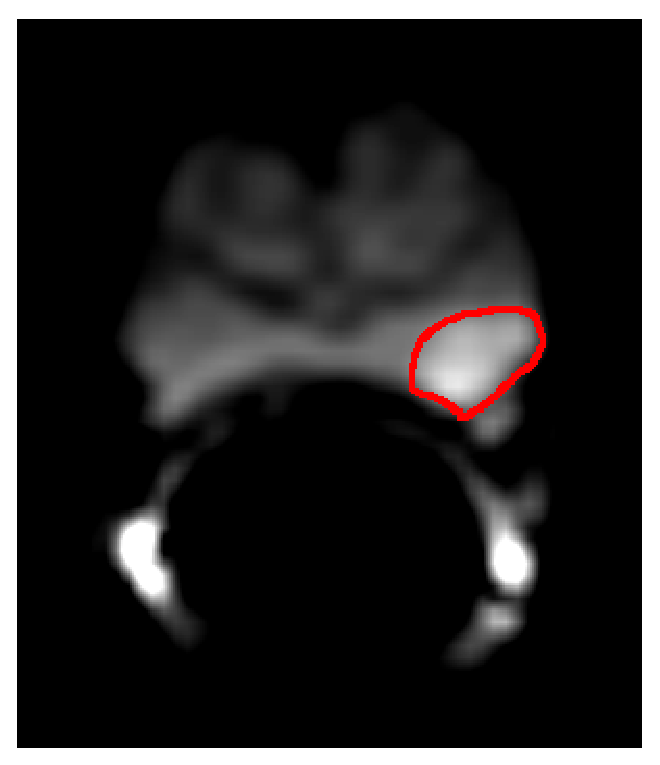
\includegraphics[width=0.25\linewidth]{2_modality/figures/dwi/dwi_cancer.eps}}
  \hfill
  \subfloat[\acs*{adc} map computer after acquisition of \acs*{dw}-\acs*{mri}
  images with \SI{1.5}{\tesla} \acs*{mri} scanner. The cancer corresponds to
  the low \acs*{si} region highlighted in
  red.]{\label{subfig:adc}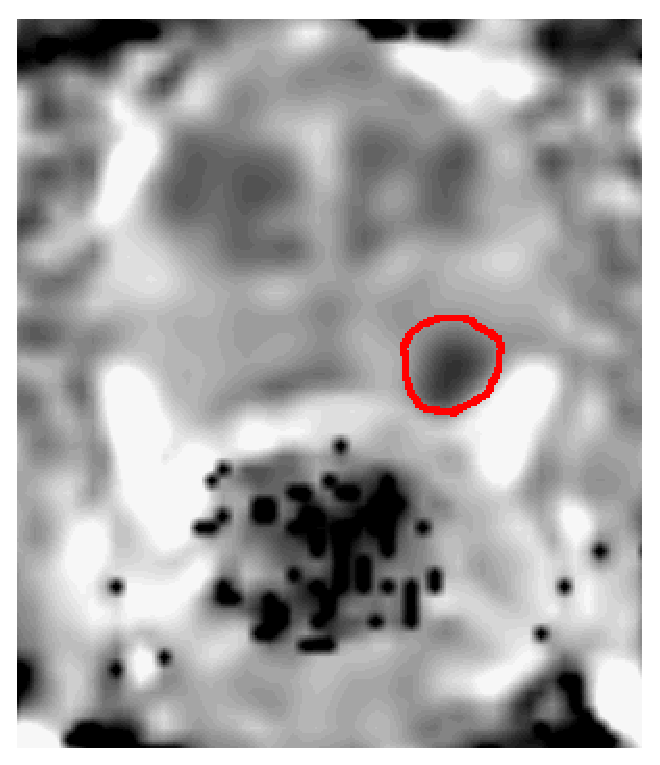
\includegraphics[width=0.25\linewidth]{2_modality/figures/dwi/adc_cancer.eps}}
  \hspace*{\fill}
  \caption[Example of \acs*{dw}-\acs*{mri} and \acs*{dce} map.]{Illustration of
    of \acs*{dw}-\acs*{mri} and \acs*{adc} map. The signal intensity
    corresponding to cancer are inversely correlated on these modalities.}
  \label{fig:dwi}
\end{figure}

\subsection{\acs*{dw}-\acs*{mri}}\label{subsec:chp2:imaging:dw}
As previously mentioned in the introduction, \ac{dw}-\ac{mri} is the most
recent \ac{mri} imaging technique aiming at \ac{cap} detection and
diagnosis~\cite{Scheidler1999}.
This modality exploits the variations in the motion of water molecules in
different tissues~\cite{LeBihan1988,Koh2007}.

The distinction between healthy and \ac{cap} in \ac{dw}-\ac{mri} is based on
the following physiological bases.
On the one hand, \ac{pz}, as previously mentioned, is mainly a glandular and
tubular structure allowing water molecules to move
freely~\cite{Choi2007,Hoeks2011}.
On the other hand, \ac{cg} is made up of muscular or fibrous tissue causing the
motion of the water molecules to be more constrained and heterogeneous than in
\ac{pz}~\cite{Hoeks2011}.
Then, \ac{cap} growth leads to the destruction of normal glandular structure
and is associated with an increase in cellular
density~\cite{Hoeks2011,Koh2007,Somford2008}.
Furthermore, these factors both have been shown to be inversely correlated with
water diffusion~\cite{Koh2007,Somford2008}: higher cellular density implies a
restricted water diffusion.
Thus, water diffusion in \ac{cap} will be more restricted than both healthy
\ac{pz} and \ac{cg}~\cite{Koh2007,Hoeks2011}.

From the \ac{nmr} principle side, \ac{dw}-\ac{mri} sequence produces contrasted
images due to variation of water molecules motion.
The method is based on the fact that the signal in \ac{dw}-\ac{mri} images is
inversely correlated to the degree of random motion of water
molecules~\cite{Huisman2003}.
In fact, gradients are used in \ac{dw}~\ac{mri} modality to encode spatial
location of nuclei temporarily.
Simplifying the problem in only one direction, a gradient is applied in that
direction, dephasing the spins of water nuclei.
Hence, the spin phases vary along the gradient direction depending of the
gradient intensity at those locations.
Then, a second gradient is applied aiming at cancelling the spin dephasing.
Thus, the immobile water molecules will be subject to the same gradient
intensity as the initial one while moving water molecules will be subject to a
different gradient intensity.
Thus, spins of moving water molecules will stay dephased whereas spins of
immobile water molecules will come back in phase.
As a consequence, a higher degree of random motion results in a more
significant signal loss whereas a lower degree of random motion is synonymous
with lower signal loss~\cite{Huisman2003}.
Under these conditions, the \ac{mri} signal is measured as:

\begin{align}
  M_{x,y}\left(t,b\right) & = M_{x,y}(0) \exp \left( - \frac{t}{\text{T}_2} \right) S_{\text{ADC}}(b) \ , \label{eq:t2dif} \\
  S_{\text{ADC}}(b) & = \exp \left( -b \times \text{ADC} \right) \ , \label{eq:dif}
\end{align}

\noindent where $S_{\text{ADC}}$ refers to signal drop due to diffusion effect,
$\text{ADC}$ is the \acl{adc}, and $b$ is the attenuation coefficient depending
only on of the gradient intensity and the gradient duration~\cite{LeBihan1986}.

By using this formulation, image acquisition with a parameter $b$ equal to
\SI{0}{\second\per\milli\metre\squared} corresponds to a \ac{t2w}-\ac{mri}
acquisition.
Then, increasing the attenuation coefficient $b$ --- i.e., increase gradient
intensity and duration --- enhances the contrast in \ac{dw}-\ac{mri} images.

To summarize, in \ac{dw}-\ac{mri}, \acp{cap} are characterized by
high-\ac{si} compared to normal tissues in \ac{pz} and \ac{cg} as shown in
\acs{fig}\,\ref{subfig:dwi}~\cite{Barentsz2012}.
However, some tissues in \ac{cg} looks similar to \ac{cap} with higher
\ac{si}~\cite{Barentsz2012}.

Diagnosis using \ac{dw}-\ac{mri} combined with \ac{t2w}-\ac{mri} has shown a
significant improvement compared with \ac{t2w}-\ac{mri} alone and provides
highly contrasted images~\cite{Shimofusa2005,Padhani2011,Choi2007}.
As drawbacks, this modality suffers from poor spatial resolution and
specificity due to false positive detection~\cite{Choi2007}.
With a view to eliminate these drawbacks, radiologists use quantitative maps
extracted from \ac{dw}-\ac{mri}, which is presented in the next section.

\subsection{\acs*{adc} map}\label{subsec:chp2:imaging:adc}
The \ac{nmr} signal measured for \ac{dw}-\ac{mri} images is not only affected
by diffusion as shown in \acs{eq}\,\eqref{eq:t2dif}.
However, the signal drop --- \acs{eq}\,\eqref{eq:dif} --- is formulated such
that the only variable is the acquisition parameter $b$~\cite{LeBihan1986}.
The \ac{adc} is considered as a ``pure'' diffusion coefficient and is extracted
to build a quantitative map known as the \acs{adc} map.
From \acs{eq}\,\eqref{eq:t2dif}, it is clear that performing multiple
acquisitions only varying $b$ will not have any effect on the term  $M_{x,y}(0)
\exp \left( - \frac{t}{\text{T}_2} \right)$.
Thus, \acs{eq}\,\eqref{eq:t2dif} can be rewritten as:

\begin{equation}
  S(b) = S_0 \exp \left( -b \times \text{ADC} \right) \ .
  \label{eq:t2adcrew}
\end{equation}

To compute the \ac{adc} map, a minimum of two acquisitions are necessary: (i)
for $b$ equal to \SI{0}{\second\per\milli\metre\squared} where the measured
signal is equal to $S_0$, and (ii) $b_1$ greater than
\SI{0}{\second\per\milli\metre\squared}, typically
\SI{1000}{\second\per\milli\metre\squared}.
Then, the \ac{adc} map can be computed as:

\begin{equation}
  \text{ADC} = - \frac{\ln \left( \cfrac{S(b_1)}{S_0} \right) }{b_1} \ .
  \label{eq:adcres1}
\end{equation}

More accurate \ac{adc} maps are computed by acquiring a set of images with
different values for the parameter $b$ and fitting linearly a semi-logarithm
function using the model presented in \acs{eq}\,\eqref{eq:t2adcrew}.

Regarding the appearance of the \ac{adc} maps, it has been previously stated
that by increasing the value of $b$, the signal of \ac{cap} tissue increases
significantly.
Considering \acs{eq}\,\eqref{eq:adcres1}, the tissue appearance in the \ac{adc}
map is the inverse of \ac{dw}-\ac{mri} images.
Then, \ac{cap} tissue is associated with low-\ac{si} whereas healthy tissue
appears brighter as depicted in
\acs{fig}\,\ref{subfig:adc}~\cite{Barentsz2012}.

Similar to the gain achieved by \ac{dw}-\ac{mri}, diagnosis using \ac{adc} map
combined with \ac{t2w}-\ac{mri} significantly outperforms \ac{t2w}-\ac{mri}
alone~\cite{Doo2012,Choi2007}.
Moreover, it has been shown that \ac{adc} coefficient is correlated with
\ac{gs}~\cite{Hambrock2011,Itou2011,Peng2013}.

However, some tissues of the \ac{cg} mimic \ac{cap} with
low-\ac{si}~\cite{Kirkham2006} and image distortion can arise due to
hemorrhage~\cite{Choi2007}.
It has also been noted that a high variability of the \ac{adc} occurs between
different patients making it difficult to define a static threshold to
distinguish \ac{cap} from non-malignant tumours~\cite{Choi2007}.

\begin{figure}
  \centering
  \hspace*{\fill}
  \subfloat[Illustration of an \acs*{mrsi} spectrum of a healthy voxel acquired
  with a \SI{3}{\tesla}
  \acs*{mri}.]{\label{subfig:mrsihea}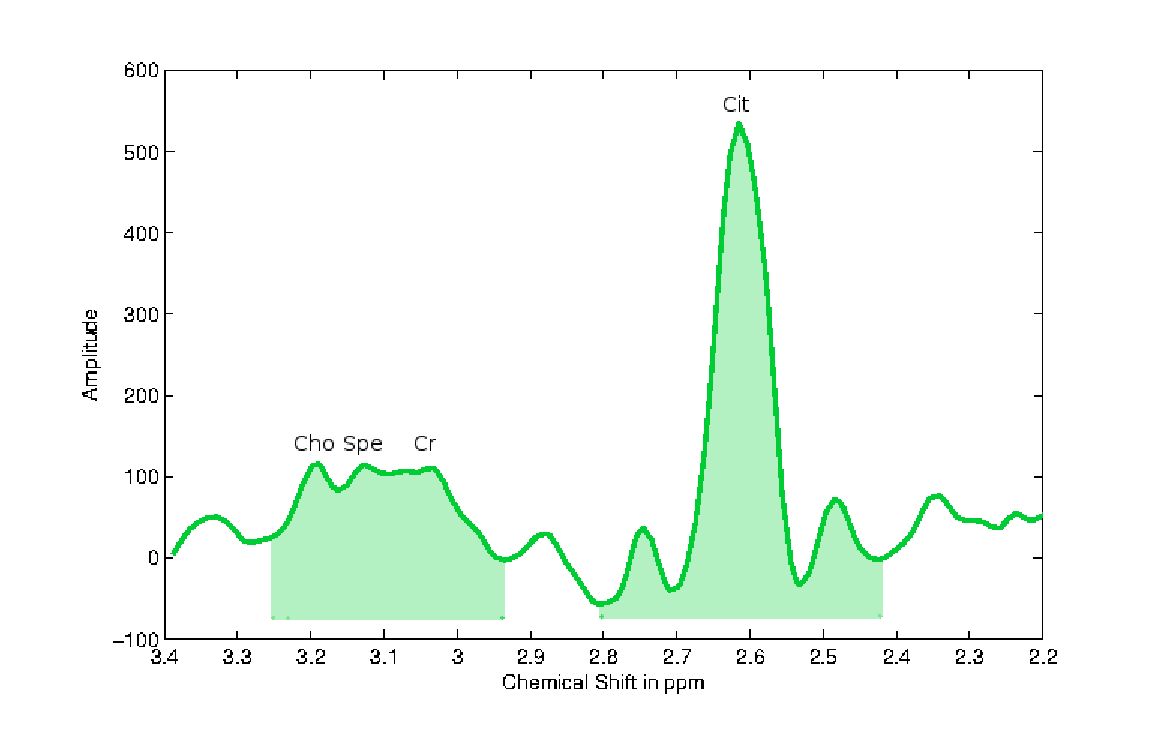
\includegraphics[width=0.45\linewidth]{2_modality/figures/mrsi/mrsi_healthy.eps}}
  \hfill
  \subfloat[Illustration of an \acs*{mrsi} spectrum of a cancerous voxel
  acquired with a \SI{3}{\tesla}
  \acs*{mri}.]{\label{subfig:mrsican}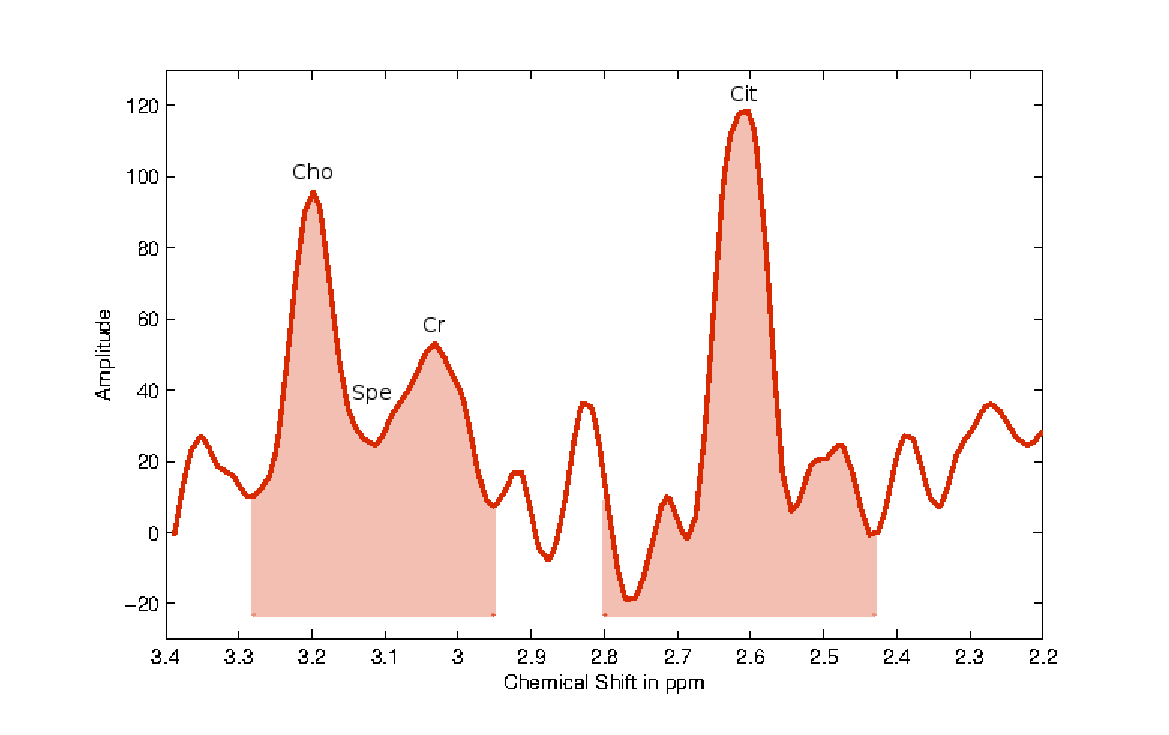
\includegraphics[width=0.45\linewidth]{2_modality/figures/mrsi/mrsi_cancer.eps}}
  \hspace*{\fill}
  \caption[Illustration of healthy and cancerous \acs*{mrsi}
  spectrum.]{Illustration of an \acs*{mrsi} spectrum for both healthy and
    cancerous voxels with a \SI{3}{\tesla} \acs*{mri}. The highlighted areas
    correspond to the related concentration of the metabolites which is
    computed by integrating the area under each peak. Acronyms: choline (Cho),
    spermine (Spe), creatine (Cr) and citrate (Cit).}
  \label{fig:mrsi}
\end{figure}

\subsection{\acs*{mrsi}}\label{subsec:chp2:imaging:mrsi}
\ac{cap} induces metabolic changes in the prostate compared with healthy tissue.
Thus, \ac{cap} detection can be carried out by tracking changes of metabolite
concentration in prostate tissue.
\ac{mrsi} is an \ac{nmr}-based technique which generates spectra of relative
metabolite concentration in \iac{roi}.

In order to track changes of metabolite concentration, it is important to know
which metabolites are associated with \ac{cap}.
To address this question, clinical studies identified three biological markers:
(i) citrate, (ii) choline, and (iii) polyamines composed mainly of spermine,
and in less abundance of spermidine and
putrescine~\cite{Awwad2012,Costello2006,Giskeodegard2013}.

Citrate is involved in the production and secretion of the prostatic fluid, and
the glandular prostate cells are associated with a high production of citrate
enabled by zinc accumulation by these same cells~\cite{Costello2006}.
However, the metabolism allowing the accumulation of citrate requires a large
amount of energy~\cite{Costello2006}.
In contrast, malignant cells do not have high zinc levels leading to lower
citrate levels due to citrate oxidization~\cite{Costello2006}.
Furthermore, this change results in a more energy-efficient metabolism enabling
malignant cells to grow and spread~\cite{Costello2006}.

An increased concentration of choline is related to \ac{cap}~\cite{Awwad2012}.
Malignant cell development requires epigenetic mechanisms resulting in
metabolic changes and relies on two mechanisms: \ac{dna} methylation and
phospholid metabolism which both result in choline uptake, explaining its
increased level in \ac{cap} tissue~\cite{Awwad2012}.
Spermine is also considered as a biological marker in
\ac{cap}~\cite{Graaf2000,Giskeodegard2013}.
In \ac{cap}, reduction of the ductal volume due to shifts in polyamine
homeostasis might lead to a reduced spermine concentration~\cite{Graaf2000}.

To determine the concentration of these biological markers, one has to focus on
the \ac{mrsi} modality.
In theory, in presence of a homogeneous magnetic field, identical nuclei
precesses at the same operating frequency known as the Lamor
frequency~\cite{Haacke1999}.
However, \ac{mrsi} is based on the fact that identical nuclei will slightly
precess at different frequencies depending on the chemical environment in which
they are immersed~\cite{Haacke1999}, a phenomenon known as the
\ac{cse}~\cite{Parfait2010}.
Given this property, metabolites are identified and their concentrations are
determined.
In this regard, the Fourier transform is used to obtain the frequency spectrum
of the \ac{nmr} signal~\cite{Haacke1999,Parfait2010}.
In this spectrum, each peak is associated with a particular metabolite and the
area under each peak corresponds to the relative concentration of this
metabolite, as illustrated in \acs{fig}\,\ref{fig:mrsi}~\cite{Parfait2010}.

Two different quantitative approaches are used to decide whether or not the
spectra of \iac{roi} is associated with \ac{cap}: (i) relative quantification
or (ii) absolute quantification~\cite{Lemaitre2011}.
In relative quantification, the ratio of choline-polyamines-creatine to citrate
is computed.
The integral of the signal is computed from choline to creatine --- i.e., from
\SIrange{3.21}{3.02}{\ppm} --- because the peaks in this region can be merged
at clinical magnetic field strengths~\cite{Hoeks2011,Graaf2000}, as depicted in
\acs{fig}\,\ref{fig:mrsi}).
Considering the previous assumptions that choline concentration rises and
citrate concentration decreases in the presence of \ac{cap}, the ratio computed
should be higher in malignant tissue than in healthy tissue.

In contrast with relative quantification, absolute quantification measures
molar concentrations by normalizing relative concentrations using water as
reference~\cite{Lemaitre2011}.
In this case, ``true'' concentrations are directly used to differentiate
malignant from healthy tissue.
However, this method is not commonly used as it requires an additional step of
acquiring water signals, inducing time and cost acquisition constraints.

\ac{mrsi} allows examination with high specificity and sensitivity compared to
other \ac{mri} modalities~\cite{Choi2007}.
Furthermore, it has been shown that combining \ac{mrsi} with \ac{mri} improves
detection and diagnosis
performance~\cite{Scheidler1999a,Kaji1998,Vilanova2009}.
Citrate and spermine concentrations are inversely correlated with the \ac{gs}
allowing us to distinguish low- from high- grade
\acp{cap}~\cite{Giskeodegard2013}.
However, choline concentration does not provide the same
properties~\cite{Giskeodegard2013}.

Unfortunately, \ac{mrsi} also presents several drawbacks.
First, \ac{mrsi} acquisition is time consuming which prevents this modality
from being used in daily clinical practise~\cite{Barentsz2012}.
In addition, \ac{mrsi} suffers from low spatial resolution due to the fact that
\ac{snr} is linked to the voxel size.
However, this issue is addressed by developing new scanners with higher
magnetic field strengths such as \SI{7.5}{\tesla}~\cite{Giskeodegard2013}.
Finally, a high variability of the relative concentrations between patients has
been observed~\cite{Choi2007}.
The same observation has been made depending on the zones studied (ie.,
\ac{pz}, \ac{cg}, base, mid-gland, apex)~\cite{Walker2010,Lemaitre2011}.
Due to this variability, it is difficult to use a fixed threshold to
differentiate \ac{cap} from healthy tissue.

\subsection{Summary and conclusions}

\acs{tab}~\ref{tab:modmri} provides an overview of the different modalities
presented in the previous section.
Indeed, each \ac{mri} modality alone provides a different discriminative level
to distinguish \ac{cap} from healthy tissue.
A recurrent statement in the literature is, however, the ability to combine
these \ac{mri} modalities would lead to the best diagnosis performance.
In this regard, we will present in the next chapter automatic tools which have
been developed to design \ac{mpmri} \ac{cad} systems for the detection of
\ac{cap}.

\begin{table}
  \scriptsize
    \caption[Overview of the features associated with each \acs*{mri} modality
    used for medical diagnosis by radiologists.]{Overview of the features
      associated with each \acs*{mri} modality used for medical diagnosis by
      radiologists. Acronyms: \acf{cap} - \acf{si} -
      \acf{gs}.}\label{tab:modmri}
    \begin{threeparttable}
      \centering
      \noindent
      \begin{tabularx}{\linewidth}{@{} l X X X l @{}}
        \toprule
        \textbf{Modality} & \textbf{Significant features} & \textbf{\acs*{cap}}
        & \textbf{Healthy tissue} & \textbf{\acs*{gs} correlation} \\
        \midrule
        \acs*{t2w}-\acs*{mri} & \acs*{si} & low-\acs*{si} in
        \acs*{pz}~\cite{Hricak1987} & intermediate to high-\acs*{si} in
        \acs*{pz}~\cite{Hricak1987} & +~\cite{Wang2008} \\
        & Shape & round or ill-defined mass in \acs*{pz}~\cite{Hricak1983} &  &
        0 \\
        & \acs*{si} & low-\acs*{si} in \acs*{cg}~\cite{Akin2006,Barentsz2012} &
        low-\acs*{si} in \acs*{cg}~\cite{Akin2006,Barentsz2012} & 0 \\
        & Shape & homogeneous mass with ill-defined edges in \acs*{cg}~\cite{Akin2006, Barentsz2012} &  & 0 \\ \\
        T$_2$ map & \acs*{si} & low-\acs*{si}~\cite{Liney1996,Gibbs2001} &
        intermediate to high-\acs*{si}~\cite{Liney1996,Gibbs2001} &
        +~\cite{Liu2011,Liney1996,Liney1997}  \\ \\
        \acs*{dce} \acs*{mri} & Semi-quantitative features~\cite{Verma2012}: &
        & & \\
        & $\bullet$ wash-in & faster & slower & 0 \\
        & $\bullet$ wash-out & faster & slower & 0 \\
        & $\bullet$ integral under the curve & higher & lower & 0 \\
        & $\bullet$ maximum signal intensity & higher & lower & 0 \\
        & $\bullet$ time-to-peak enhancement & faster & slower & 0 \\ \\
        & Quantitative features (Tofts' parameters~\cite{Tofts2010}): & & & \\
        & $\bullet$ $\text{k}_{\text{ep}}$ & higher & lower & 0 \\
        & $\bullet$ $\text{K}^{\text{trans}}$ & higher & lower & 0 \\ \\
        \acs*{dw} \acs*{mri} & \acs*{si} &
        higher-\acs*{si}~\cite{Huisman2003,Barentsz2012} &
        lower-\acs*{si}~\cite{Huisman2003,Barentsz2012} & + \\ \\
        \acs*{adc} map & \acs*{si} & low-\acs*{si}~\cite{Barentsz2012} &
        high-\acs*{si}~\cite{Barentsz2012} & +~\cite{Hambrock2011, Itou2011,
          Peng2013} \\ \\
        \acs*{mrsi}& Metabolites: & & & \\
        & $\bullet$ citrate (2.64 ppm)~\cite{Verma2010} & lower
        concentration~\cite{Awwad2012,Costello2006,Graaf2000} & higher
        concentration~\cite{Awwad2012,Costello2006,Graaf2000} &
        +~\cite{Giskeodegard2013} \\
        & $\bullet$ choline (3.21 ppm)~\cite{Verma2010} & higher
        concentration~\cite{Awwad2012,Costello2006,Graaf2000} & lower
        concentration~\cite{Awwad2012,Costello2006,Graaf2000} &
        0~\cite{Giskeodegard2013} \\
        & $\bullet$ spermine (3.11 ppm)~\cite{Verma2010} & lower
        concentration~\cite{Awwad2012,Costello2006,Graaf2000} & higher
        concentration~\cite{Awwad2012,Costello2006,Graaf2000} &
        +~\cite{Giskeodegard2013} \\
        \bottomrule
      \end{tabularx}
      \begin{tablenotes}
      \item Notes:
      \item + = significantly correlated;
      \item 0 = no correlation.
      \end{tablenotes}
    \end{threeparttable}
  \label{tab:modmri}
\end{table}

